\paragraph*{Node addition} We demonstrate how we can add nodes.
Essentially, ensure the user is in mouse mode, hold A and press left click to place the node,
as seen in the figures \ref{fig:app:node-addition}.
We observe in figure \ref{fig:chap-5:full-add} that the \textsc{Copy} gate
is circled in pink to denote invalid arity, meaning its missing its input
and output edge. In addition, hovering over a node
will highlight the node in yellow as seen in figure \ref{fig:app:full-toggle}.

\begin{figure}[htbp]
    \centering
    \subfloat[Holding A gives an indicator of where the node will be placed]{
        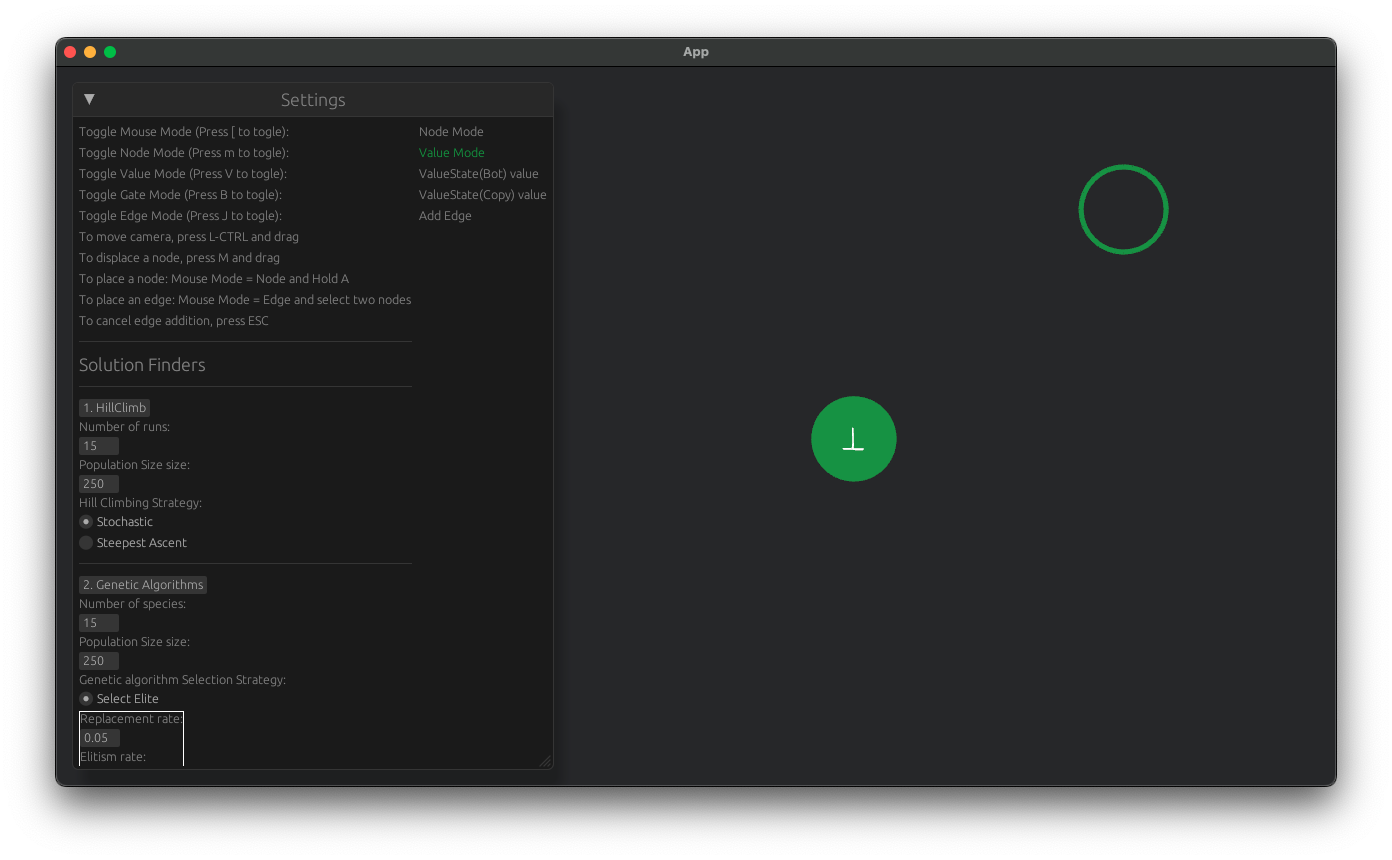
\includegraphics[width=0.5\linewidth]{Appendices/user-storynode-add.png}
        \label{fig:app:hold-add}
    }
    \subfloat[Final graph after addition of values and gate nodes]{
        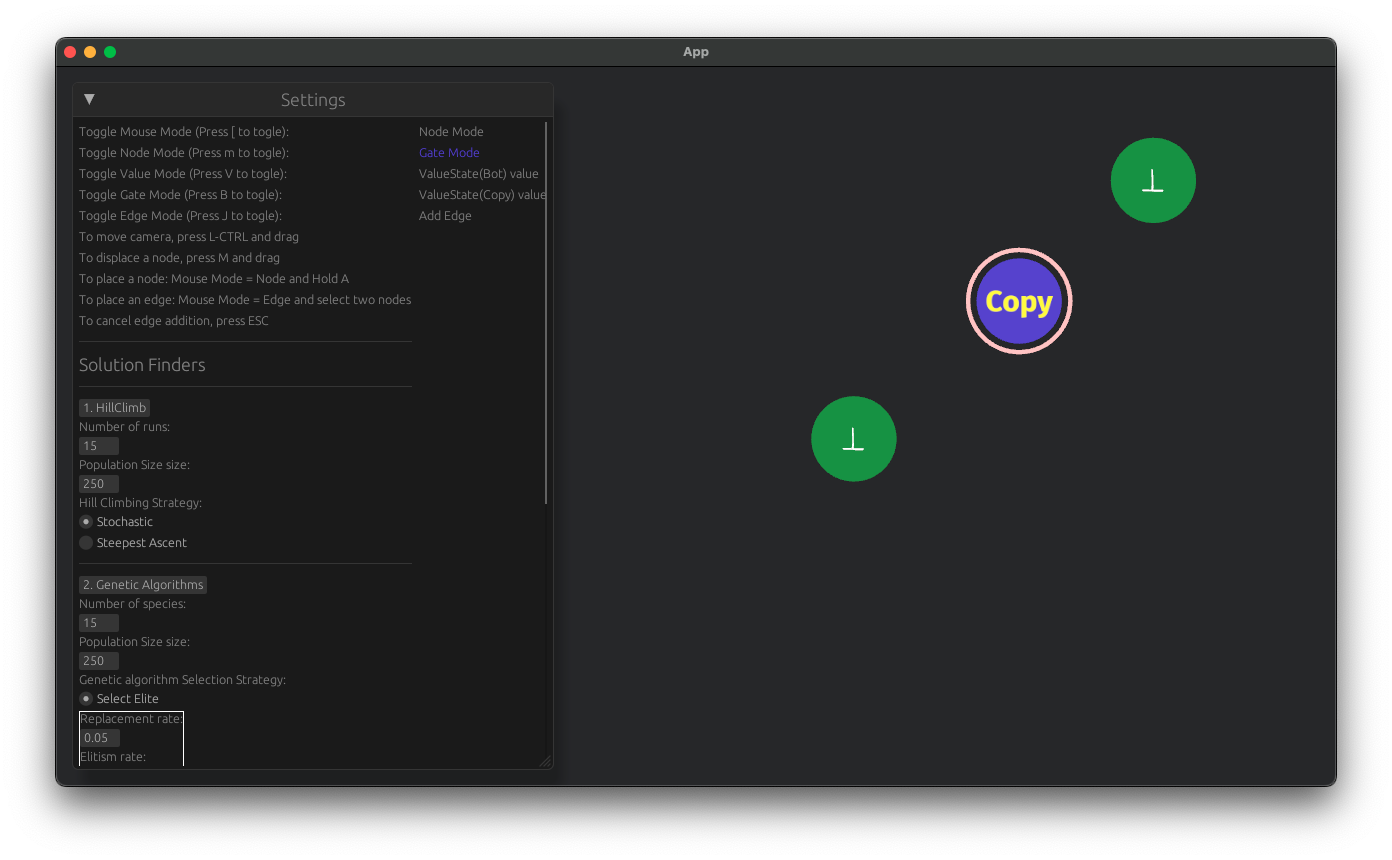
\includegraphics[width=0.5\linewidth]{Appendices/user-story-node-add-invalid-arity.png}
        \label{fig:chap-5:full-add}
    }
    \caption{Node addition}
    \label{fig:app:node-addition}
\end{figure}


\FloatBarrier
\paragraph*{Edge addition} To add an edge
between two nodes, we select the source of the edge.
We can observe from the figure \ref{fig:app:hold-edge}, that we highlight the source node
with light blue and the
heterogeneous nodes with orange. If we select a gate, we highlight only
nodes have an in-degree of $0$.
Pressing ESC or changing mode can cancel the selection operation.
Selecting on any of the orange nodes completes
the edge addition operation as seen in figure \ref{fig:app:some-add}. We can also observe that since the \textsc{Copy} has
no error circles since it has the correct arity and the input/output values satisfy the gate as seen in \ref{fig:app:full-add}.


\begin{figure}[htbp]
    \centering

    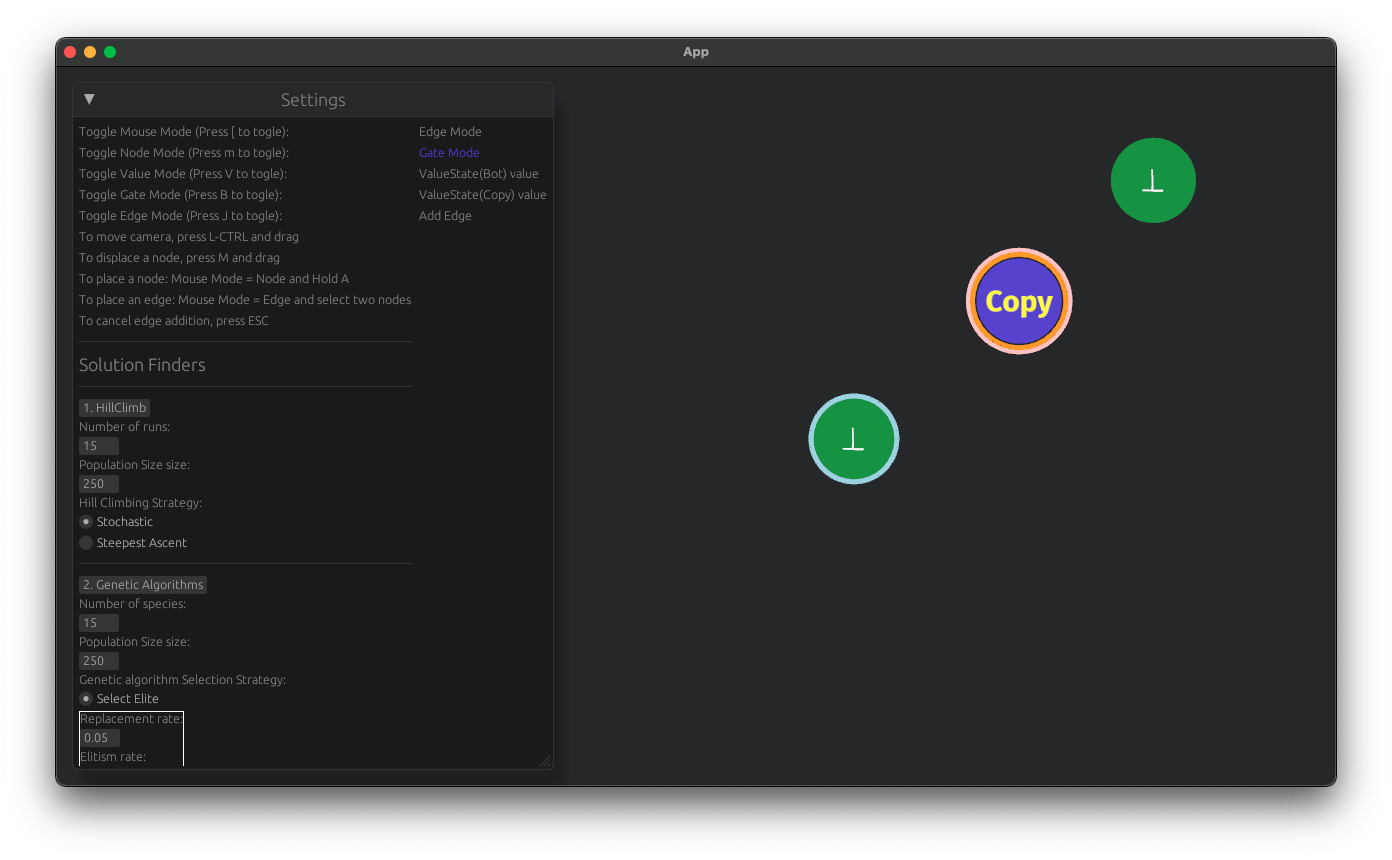
\includegraphics[width=0.7\linewidth]{Appendices/user-story-add-edge-highlight.png}
    \caption{Edge addition: Select source node}
    \label{fig:app:hold-edge}

\end{figure}
\begin{figure}[htbp]
    \centering

    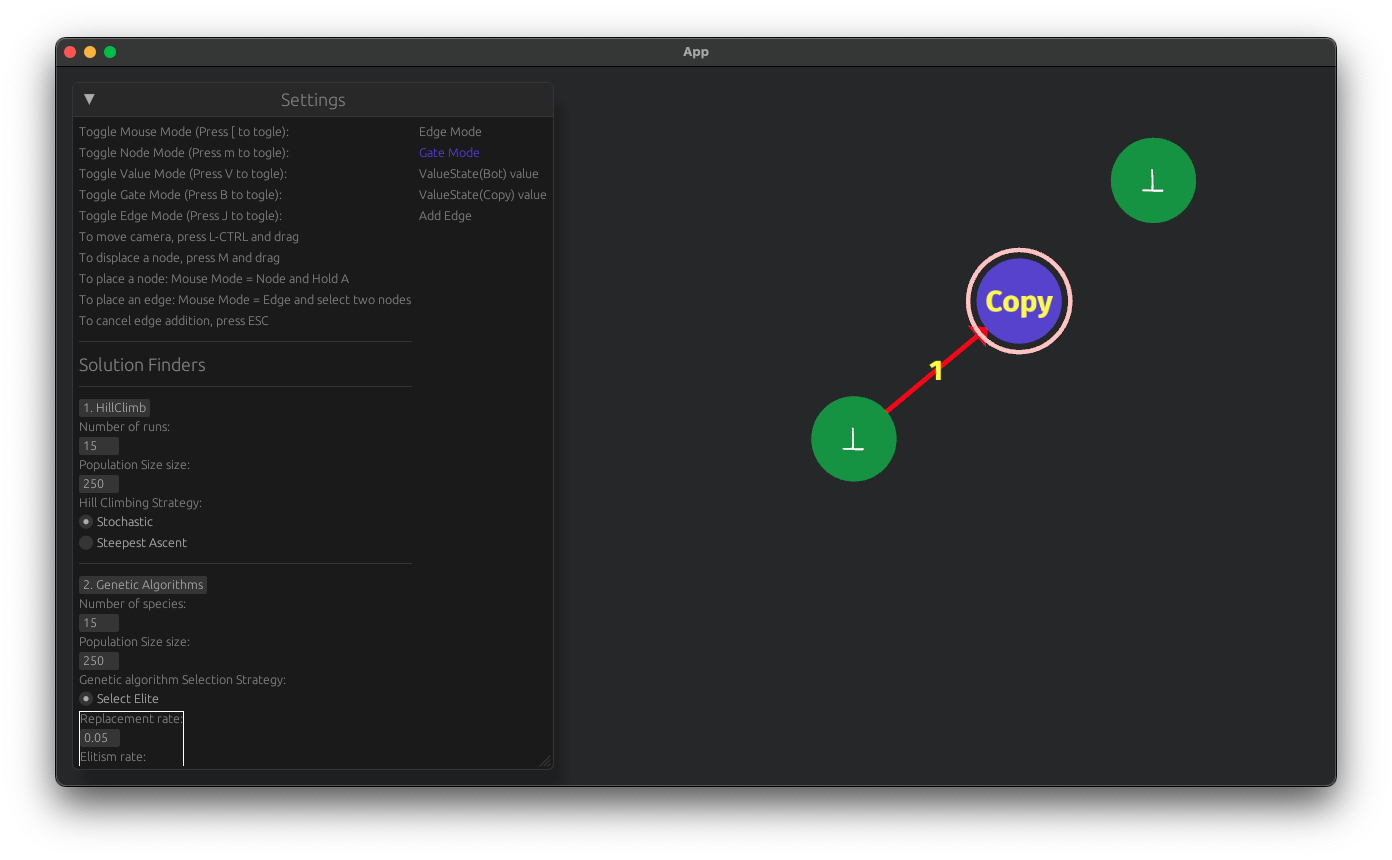
\includegraphics[width=0.7\linewidth]{Appendices/users-story-finish-add.png}
    \caption{Edge addition: Select destination node}
    \label{fig:app:some-add}

\end{figure}
\begin{figure}[htbp]
    \centering

    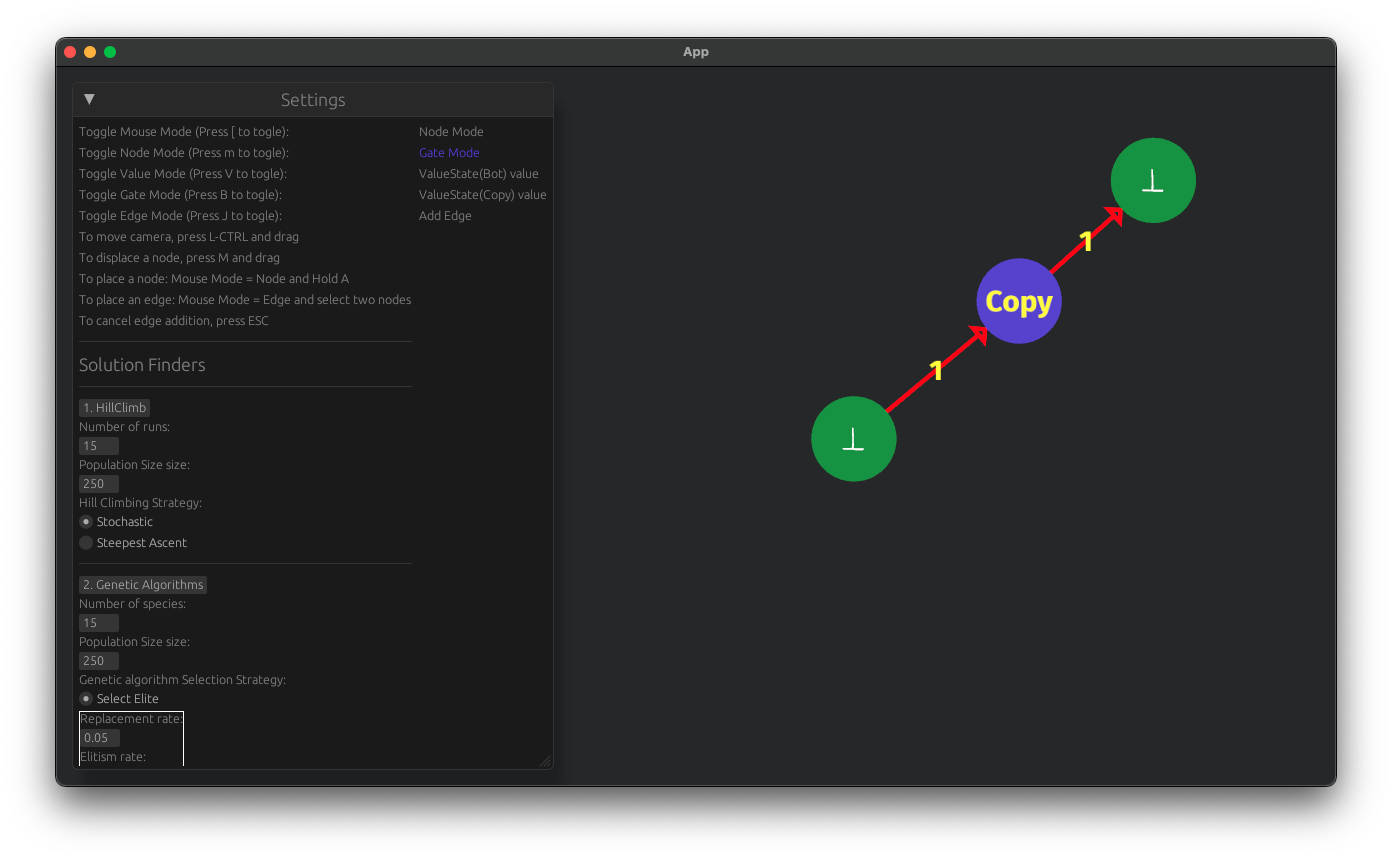
\includegraphics[width=0.7\linewidth]{Appendices/user-story-full-edge.png}
    \caption{Full graph with edges}
    \label{fig:app:full-add}
\end{figure}
\FloatBarrier
\begin{figure}[htbp]
    \centering

    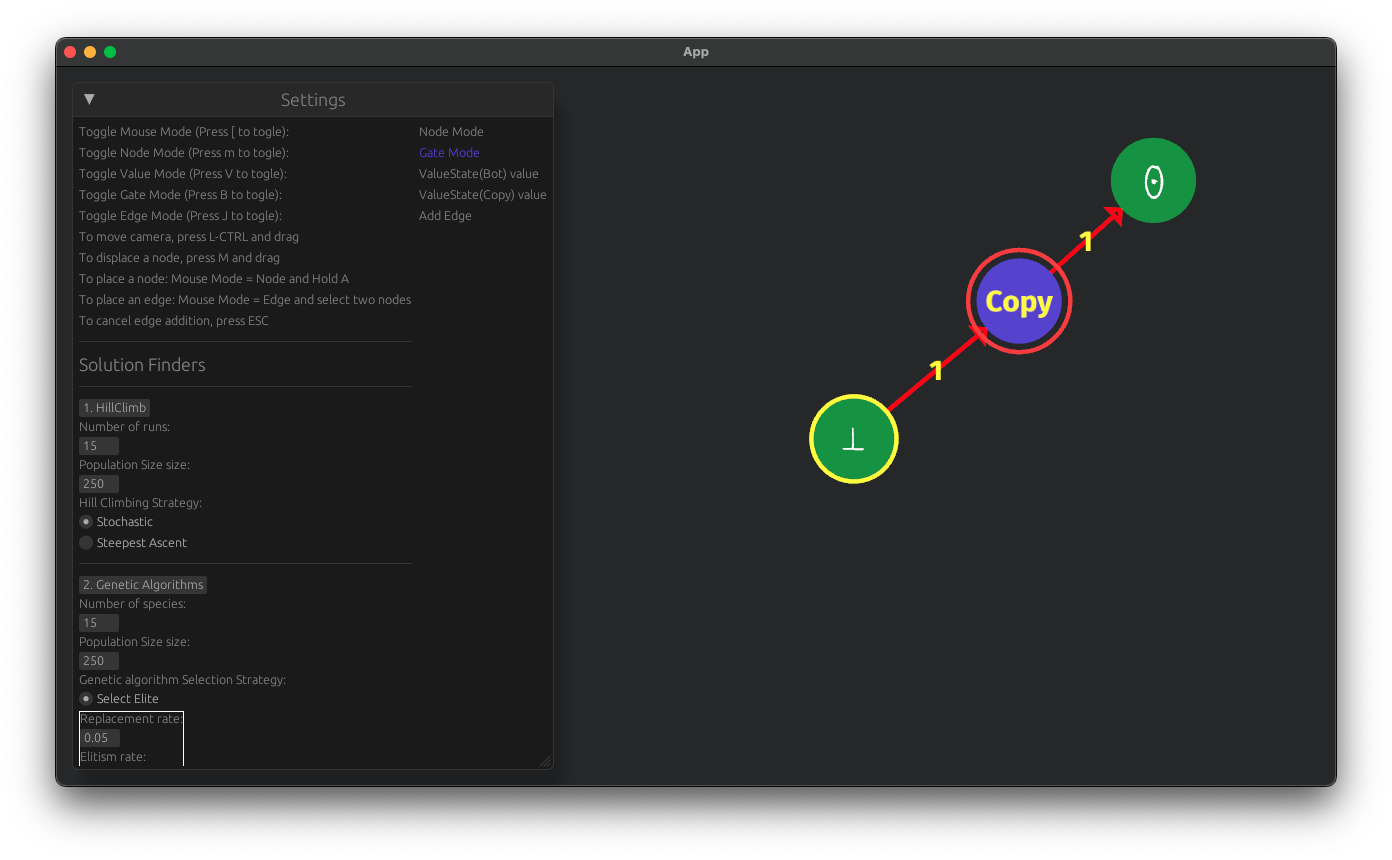
\includegraphics[width=0.7\linewidth]{Appendices/user-story-node-hover.png}
    \caption{Value node toggle and node hover}
    \label{fig:app:full-toggle}
\end{figure}
\FloatBarrier

\paragraph*{Node/Edge deletion}

To delete nodes we can simplify hover over a node and press D. For edge deletion
the procedure is the same as the edge addition, but we can only select nodes that are incident
to our current node. We provide examples in \ref{fig:app:node-rem} and \ref{fig:app:edge-rem}

\begin{figure}[htbp]
    \centering
    \subfloat[Node removal: Before removal]{
        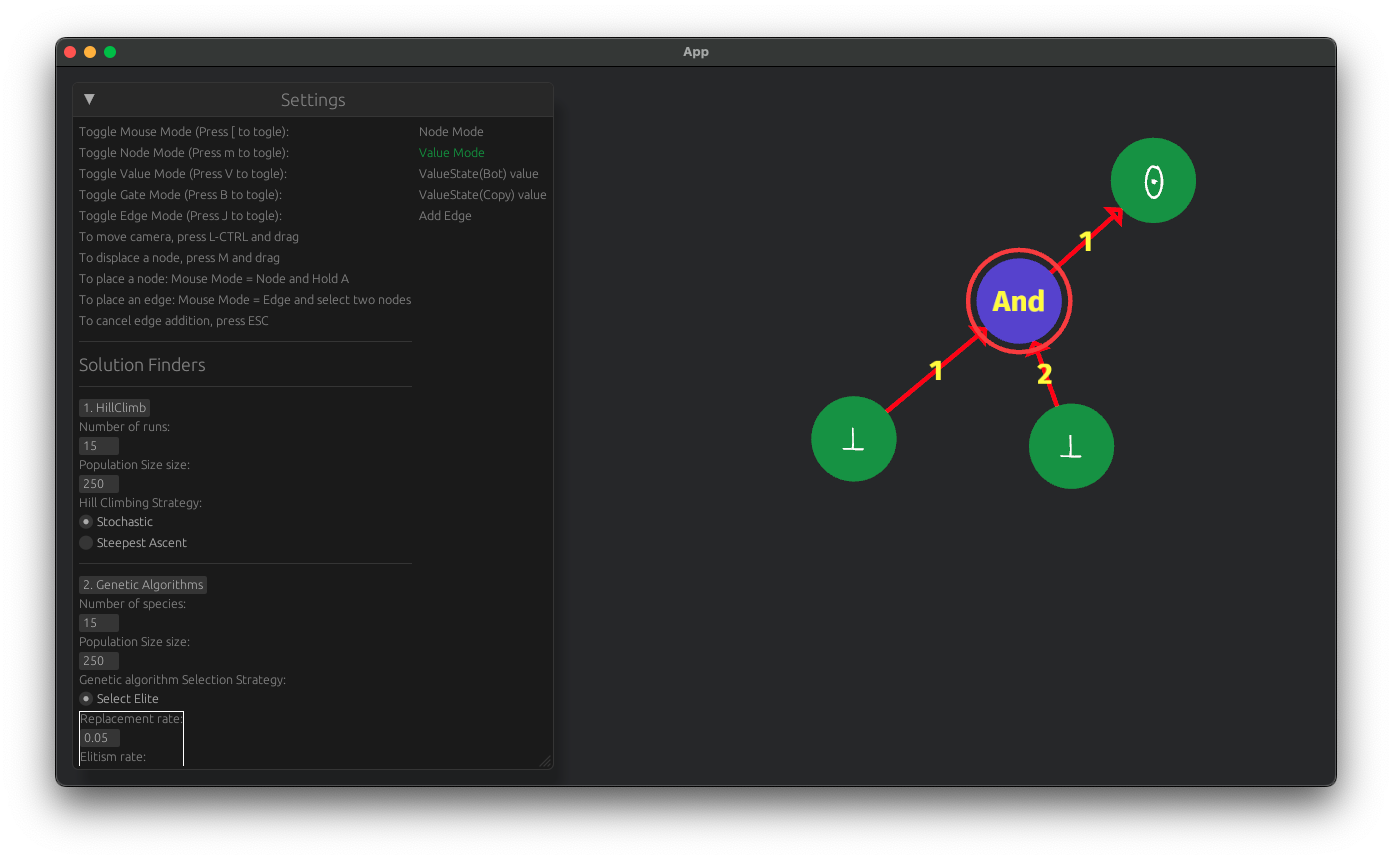
\includegraphics[width=0.5\linewidth]{Appendices/user-story-before-nod-rem.png}
        \label{fig:app:before-node-rem}
    }
    \subfloat[Node removal: After removal]{
        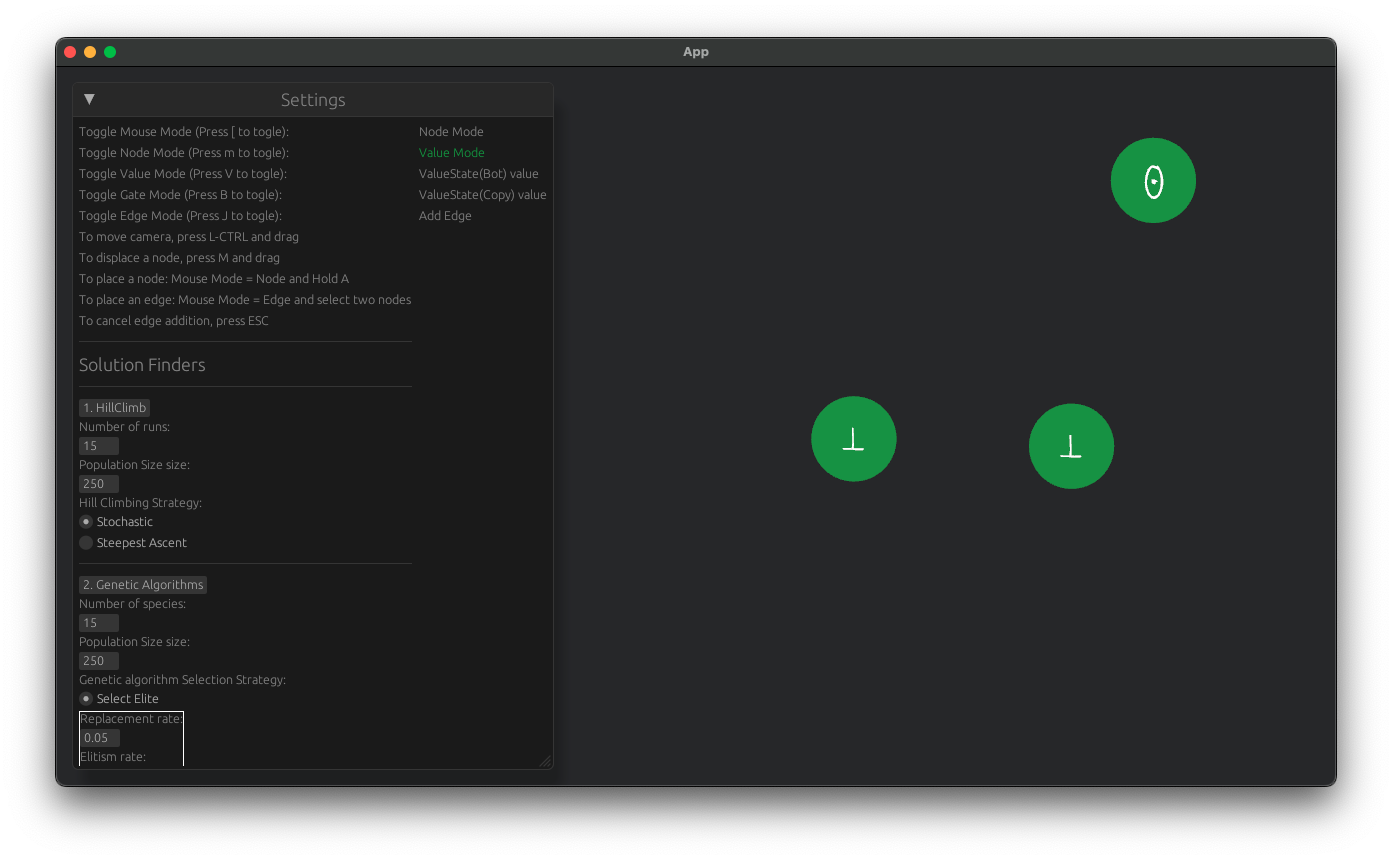
\includegraphics[width=0.5\linewidth]{Appendices/user-story-after-node-rem.png}
        \label{fig:app:after-node-rem}
    }
    \caption{Node removal}
    \label{fig:app:node-rem}
\end{figure}


\begin{figure}[htbp]
    \centering
    \subfloat[Edge removal: Before removal]{
        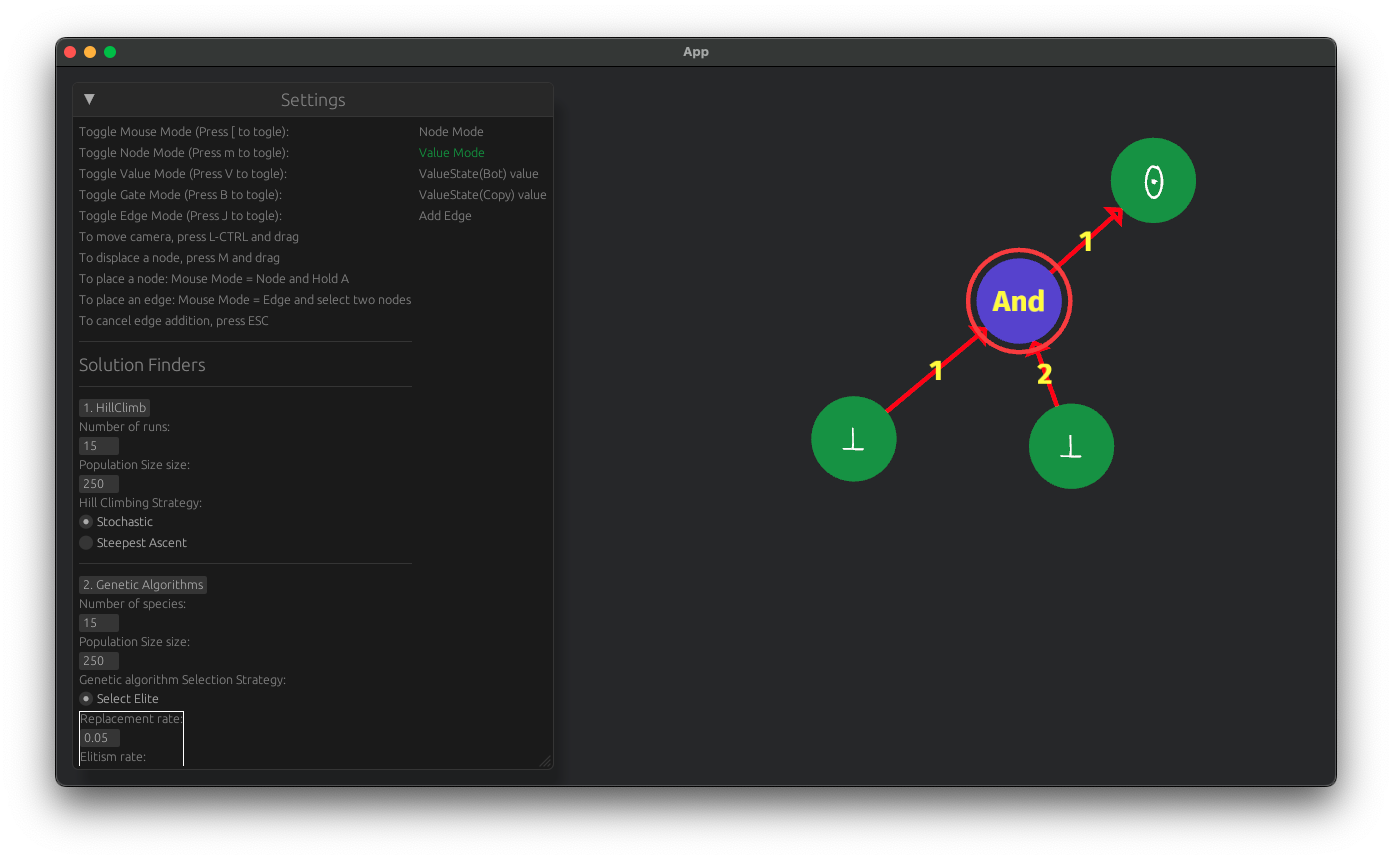
\includegraphics[width=0.5\linewidth]{Appendices/user-story-before-nod-rem.png}
        \label{fig:app:before-edge-rem}
    }
    \subfloat[Edge removal: After removal]{
        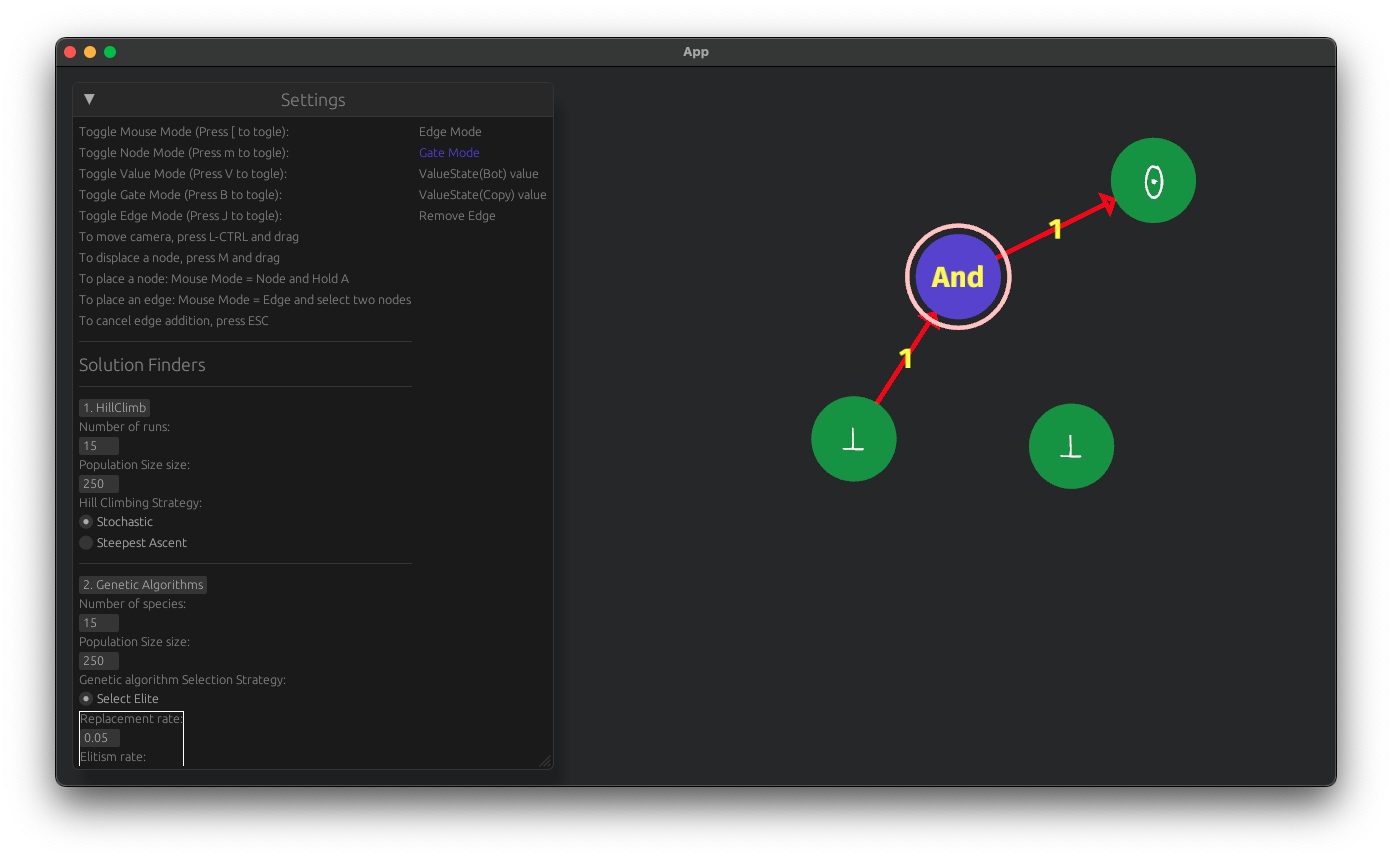
\includegraphics[width=0.5\linewidth]{Appendices/user-story-after-edge-rem.png}
        \label{fig:app:after-edge-rem}
    }
    \caption{Edge removal}
    \label{fig:app:edge-rem}
\end{figure}
\FloatBarrier

% \begin{figure}[htbp]
%     \centering
%     \subfloat[Edge addition: Select source node]{
%         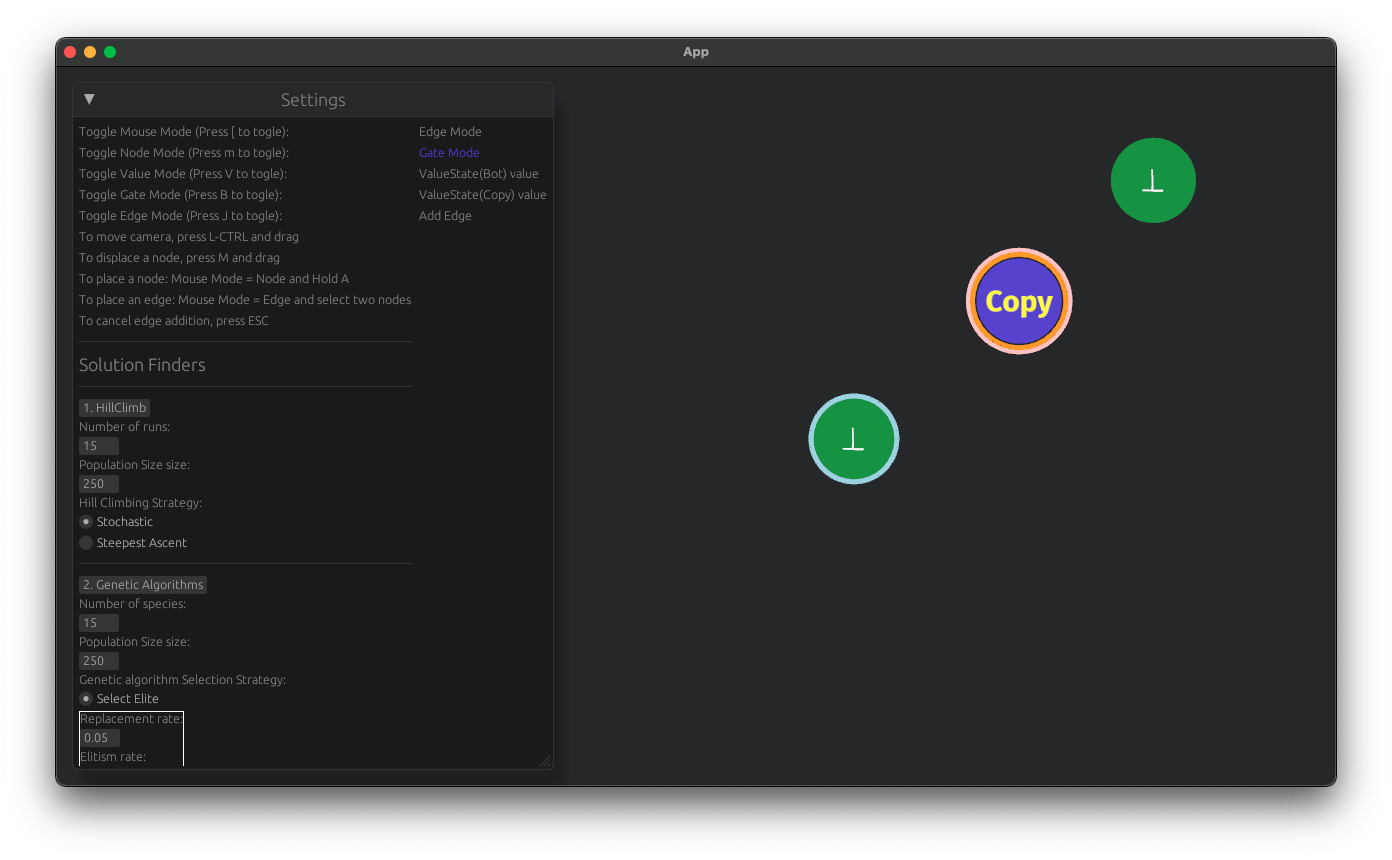
\includegraphics[width=0.5\linewidth]{Appendices/user-story-add-edge-highlight.png}
%         \label{fig:app:hold-edge}
%     }
%     \subfloat[Edge addition: Select destination node]{
%         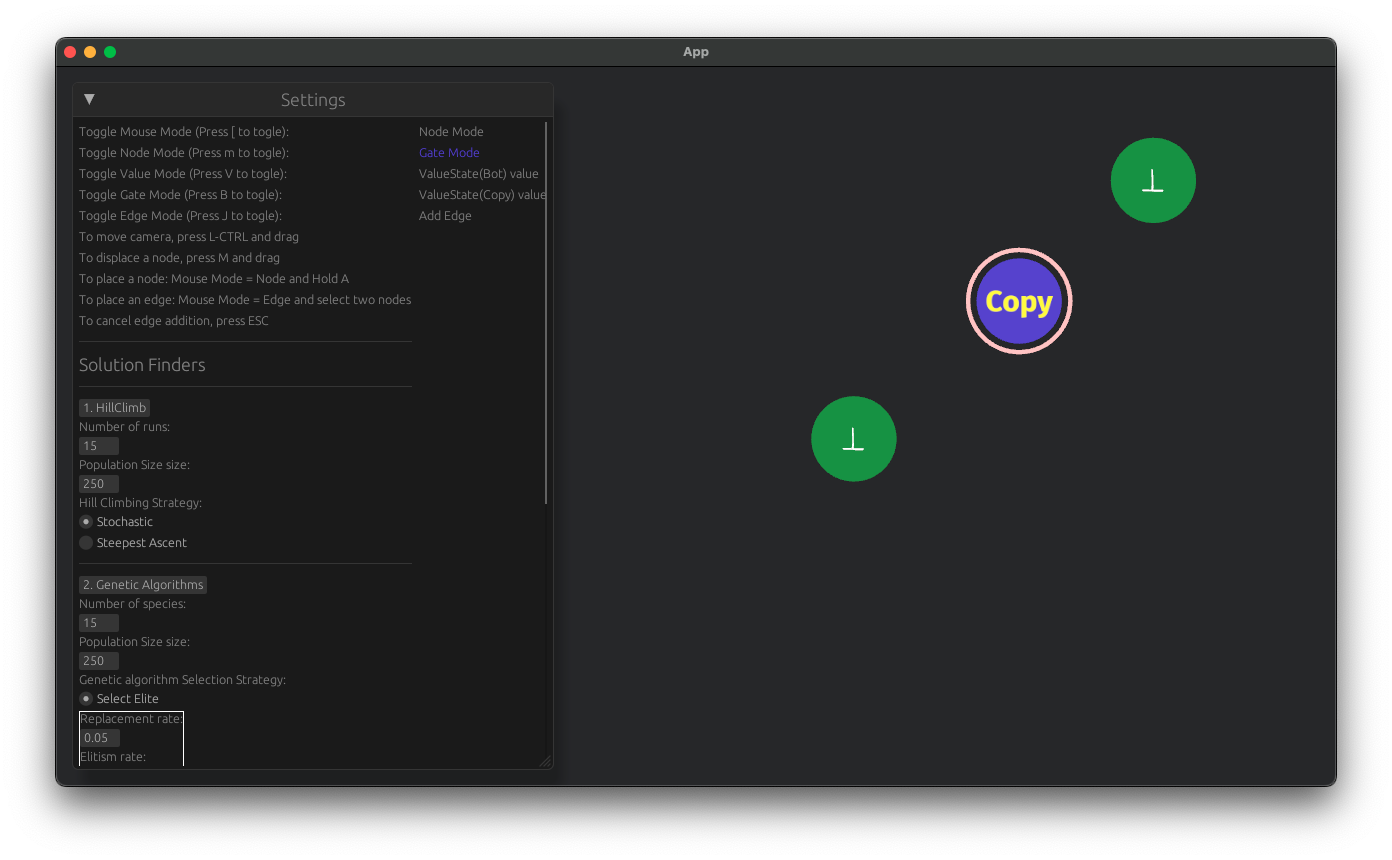
\includegraphics[width=0.5\linewidth]{Appendices/user-story-node-add-invalid-arity.png}
%         \label{fig:chap-5:some-add}
%     }
%     \caption{Node addition}
%     \label{fig:app:edge-addition}
% \end{figure}